\documentclass[11pt]{article}
%\usepackage{psfig}
\usepackage{latexsym}
\usepackage{amsfonts}
\usepackage{hyperref}
\usepackage{url}
\usepackage{listings}
% to use hyperlinks in References section
\hypersetup{urlbordercolor={1 1 1}}
\usepackage{graphicx}
\usepackage{listings}	

%define colors
\usepackage{xcolor} 	
\definecolor{dkgreen}{rgb}{0,0.6,0}
\definecolor{gray}{rgb}{0.5,0.5,0.5}
\definecolor{mauve}{rgb}{0.58,0,0.82}
\usepackage{graphicx}
\usepackage{hyperref}
\hypersetup{urlbordercolor={1 1 1}}
\DeclareGraphicsExtensions{.pdf,.jpg,.png,.eps}
\setlength{\textheight}{8.5in}
\setlength{\textwidth}{6.0in}
\setlength{\headheight}{0in}
\addtolength{\topmargin}{-.5in}
\addtolength{\oddsidemargin}{-.5in}

\usepackage{url}
\def\UrlBreaks{\do\A\do\B\do\C\do\D\do\E\do\F\do\G\do\H\do\I\do\J
\do\K\do\L\do\M\do\N\do\O\do\P\do\Q\do\R\do\S\do\T\do\U\do\V
\do\W\do\X\do\Y\do\Z\do\[\do\\\do\]\do\^\do\_\do\`\do\a\do\b
\do\c\do\d\do\e\do\f\do\g\do\h\do\i\do\j\do\k\do\l\do\m\do\n
\do\o\do\p\do\q\do\r\do\s\do\t\do\u\do\v\do\w\do\x\do\y\do\z
\do\.\do\@\do\\\do\/\do\!\do\_\do\|\do\;\do\>\do\]\do\)\do\,
\do\?\do\'\do+\do\=\do\#} 

\newenvironment{cvl}{\begin{list}{$\bullet$}{
\setlength{\leftmargin}{0.3in} \setlength{\labelsep}{0.07in}
\setlength{\labelwidth}{0.17in} \setlength{\rightmargin}{0.0in}
\setlength{\topsep}{0.000in} \setlength{\partopsep}{0.000in}
\setlength{\parskip}{0.000in} \setlength{\parsep}{0.005in}
\setlength{\itemsep}{0.005in}}}{\end{list}}

\DeclareGraphicsExtensions{.pdf,.jpg,.png,.eps}
\usepackage[T1]{fontenc}	%special characters copy-able
\usepackage{xspace}
\usepackage{times}
\usepackage{enumerate}
\newcommand{\espoofer}{{\sf espoofer}\space}
\newcommand{\dmark}{{\sf DMARC}\space}
\newcommand{\dkim}{{\sf DKIM}\space}
\newcommand{\spf}{{\sf SPF}\space}
\newcommand{\tor}{{\sf Tor}\xspace}
\newcommand{\torbw}{{\sf Tor Browser}\xspace}
\newcommand{\darkweb}{{\sf DarkWeb}\xspace}
\definecolor{myblue}{HTML}{1F5AB4}%1F5AB4
\hypersetup{colorlinks,urlcolor=black,linkcolor=myblue,anchorcolor=black,citecolor=red}
%--------------
%% Modified by Zhiqiang Lin
%% 01/18/2012
%%
%% Template file was from http://www.cs.umd.edu/~jkatz
%%
%% preamble.tex
%% this should be included with a command like
%% %--------------
%% Modified by Zhiqiang Lin
%% 01/18/2012
%%
%% Template file was from http://www.cs.umd.edu/~jkatz
%%
%% preamble.tex
%% this should be included with a command like
%% %--------------
%% Modified by Zhiqiang Lin
%% 01/18/2012
%%
%% Template file was from http://www.cs.umd.edu/~jkatz
%%
%% preamble.tex
%% this should be included with a command like
%% \input{preamble.tex}
%% \lecture{``lecture number''}{``date''}{``name of professor''}{``name
%%  of student''}

\hbadness=10000
\vbadness=10000

\newcommand{\handout}[5]{
   \renewcommand{\thepage}{#1-\arabic{page}}
   \noindent
   \begin{center}
   \framebox{
      \vbox{
    \hbox to 5.78in { {\bf CSE 5473 --- Network Security} 
     	 \hfill #2 }
       \vspace{4mm}
       \hbox to 5.78in { {\Large \hfill #5  \hfill} }
       \vspace{2mm}
       \hbox to 5.78in { {\it #3 \hfill #4} }
      }
   }
   \end{center}
   \vspace*{4mm}
}

\newcommand{\lecture}[4]{\handout{#1}{#2}{#3}{#4}{#1}}
%\newcommand{\lecture}[4]{\handout{#1}{#2}{Lecturer: #3}{Scribe(s): #4}{Lecture #1}}

\def\epsilon{\varepsilon}
\def\phi{\varphi}
\def\bool{\{0,1\}}
\def\poly{{\sf poly}}
\def\cross{\times}

\newcommand{\xor}{\oplus}
\newcommand{\Xor}{\bigoplus}
\newcommand{\ceil}[1]{\left\lceil {#1} \right\rceil}
\newcommand{\floor}[1]{\left\lfloor #1 \right\rfloor}
\newcommand{\ignore}[1]{}
\newcommand{\integers}[1]{{\mathbb Z}_{#1}}
\newcommand{\bydef}{\stackrel{\rm def}{=}}
\newcommand{\isequal}{\stackrel{\rm ?}{=}}
\newcommand{\compeq}{\stackrel{\rm c}{\equiv}} % computationally indistinguishable

\newcommand{\qed}{\hspace*{\fill}\rule{7pt}{7pt}}
\newenvironment{proof_sketch}{\noindent{\bf Sketch of Proof} (Informal)\hspace*{1em}}{\qed\medskip}
\newenvironment{proof}{\noindent{\bf Proof}\hspace*{1em}}{\qed\medskip}
\newenvironment{proofof}[1]{\noindent{\bf Proof} of #1:\hspace*{1em}}{\qed\medskip}
%\newenvironment{claim}{\noindent{\bf Claim}\hspace*{1em}\begin{em}}{\end{em}\medskip}
\newcounter{defcounter}
\setcounter{defcounter}{1}
\newenvironment{definition}{\medskip\noindent{\bf Definition \thedefcounter}}{\hspace*{\fill}$\diamondsuit$\stepcounter{defcounter}\medskip}
\newtheorem{theorem}{Theorem}
\newtheorem{corollary}[theorem]{Corollary}
\newtheorem{lemma}[theorem]{Lemma}
\newtheorem{claim}[theorem]{Claim}
\newtheorem{fact}[theorem]{Fact}
\newtheorem{conjecture}[theorem]{Conjecture}
\newenvironment{assumption}{\noindent{\bf Assumption}\hspace*{1em}\begin{em}}{\end{em}\medskip}
\newenvironment{remark}{\noindent{\bf Remark}\hspace*{1em}}{\bigskip}

\ignore{
\newcommand{\FOR}{{\bf for}}
\newcommand{\TO}{{\bf to}}
\newcommand{\DO}{{\bf do}}
\newcommand{\WHILE}{{\bf while}}
\newcommand{\AND}{{\bf and}}
\newcommand{\IF}{{\bf if}}
\newcommand{\THEN}{{\bf then}}
\newcommand{\ELSE}{{\bf else}}

%%% You probably will not need to use the commands listed below

\makeatletter
\def\fnum@figure{{\bf Figure \thefigure}}
\def\fnum@table{{\bf Table \thetable}}
\long\def\@mycaption#1[#2]#3{\addcontentsline{\csname
  ext@#1\endcsname}{#1}{\protect\numberline{\csname 
  the#1\endcsname}{\ignorespaces #2}}\par
  \begingroup
    \@parboxrestore
    \small
    \@makecaption{\csname fnum@#1\endcsname}{\ignorespaces #3}\par
  \endgroup}
\def\mycaption{\refstepcounter\@captype \@dblarg{\@mycaption\@captype}}
\makeatother

\newcommand{\figcaption}[1]{\mycaption[]{#1}}
\newcommand{\tabcaption}[1]{\mycaption[]{#1}}
\newcommand{\head}[1]{\chapter[Lecture \##1]{}}
\newcommand{\mathify}[1]{\ifmmode{#1}\else\mbox{$#1$}\fi}
\def\half{\frac{1}{2}}

\newcommand{\fig}[4]{
        \begin{figure}
        \setlength{\epsfysize}{#2}
        \vspace{3mm}
        \centerline{\epsfbox{#4}}
        \caption{#3} \label{#1}
        \end{figure}
        }
}



%% \lecture{``lecture number''}{``date''}{``name of professor''}{``name
%%  of student''}

\hbadness=10000
\vbadness=10000

\newcommand{\handout}[5]{
   \renewcommand{\thepage}{#1-\arabic{page}}
   \noindent
   \begin{center}
   \framebox{
      \vbox{
    \hbox to 5.78in { {\bf CSE 5473 --- Network Security} 
     	 \hfill #2 }
       \vspace{4mm}
       \hbox to 5.78in { {\Large \hfill #5  \hfill} }
       \vspace{2mm}
       \hbox to 5.78in { {\it #3 \hfill #4} }
      }
   }
   \end{center}
   \vspace*{4mm}
}

\newcommand{\lecture}[4]{\handout{#1}{#2}{#3}{#4}{#1}}
%\newcommand{\lecture}[4]{\handout{#1}{#2}{Lecturer: #3}{Scribe(s): #4}{Lecture #1}}

\def\epsilon{\varepsilon}
\def\phi{\varphi}
\def\bool{\{0,1\}}
\def\poly{{\sf poly}}
\def\cross{\times}

\newcommand{\xor}{\oplus}
\newcommand{\Xor}{\bigoplus}
\newcommand{\ceil}[1]{\left\lceil {#1} \right\rceil}
\newcommand{\floor}[1]{\left\lfloor #1 \right\rfloor}
\newcommand{\ignore}[1]{}
\newcommand{\integers}[1]{{\mathbb Z}_{#1}}
\newcommand{\bydef}{\stackrel{\rm def}{=}}
\newcommand{\isequal}{\stackrel{\rm ?}{=}}
\newcommand{\compeq}{\stackrel{\rm c}{\equiv}} % computationally indistinguishable

\newcommand{\qed}{\hspace*{\fill}\rule{7pt}{7pt}}
\newenvironment{proof_sketch}{\noindent{\bf Sketch of Proof} (Informal)\hspace*{1em}}{\qed\medskip}
\newenvironment{proof}{\noindent{\bf Proof}\hspace*{1em}}{\qed\medskip}
\newenvironment{proofof}[1]{\noindent{\bf Proof} of #1:\hspace*{1em}}{\qed\medskip}
%\newenvironment{claim}{\noindent{\bf Claim}\hspace*{1em}\begin{em}}{\end{em}\medskip}
\newcounter{defcounter}
\setcounter{defcounter}{1}
\newenvironment{definition}{\medskip\noindent{\bf Definition \thedefcounter}}{\hspace*{\fill}$\diamondsuit$\stepcounter{defcounter}\medskip}
\newtheorem{theorem}{Theorem}
\newtheorem{corollary}[theorem]{Corollary}
\newtheorem{lemma}[theorem]{Lemma}
\newtheorem{claim}[theorem]{Claim}
\newtheorem{fact}[theorem]{Fact}
\newtheorem{conjecture}[theorem]{Conjecture}
\newenvironment{assumption}{\noindent{\bf Assumption}\hspace*{1em}\begin{em}}{\end{em}\medskip}
\newenvironment{remark}{\noindent{\bf Remark}\hspace*{1em}}{\bigskip}

\ignore{
\newcommand{\FOR}{{\bf for}}
\newcommand{\TO}{{\bf to}}
\newcommand{\DO}{{\bf do}}
\newcommand{\WHILE}{{\bf while}}
\newcommand{\AND}{{\bf and}}
\newcommand{\IF}{{\bf if}}
\newcommand{\THEN}{{\bf then}}
\newcommand{\ELSE}{{\bf else}}

%%% You probably will not need to use the commands listed below

\makeatletter
\def\fnum@figure{{\bf Figure \thefigure}}
\def\fnum@table{{\bf Table \thetable}}
\long\def\@mycaption#1[#2]#3{\addcontentsline{\csname
  ext@#1\endcsname}{#1}{\protect\numberline{\csname 
  the#1\endcsname}{\ignorespaces #2}}\par
  \begingroup
    \@parboxrestore
    \small
    \@makecaption{\csname fnum@#1\endcsname}{\ignorespaces #3}\par
  \endgroup}
\def\mycaption{\refstepcounter\@captype \@dblarg{\@mycaption\@captype}}
\makeatother

\newcommand{\figcaption}[1]{\mycaption[]{#1}}
\newcommand{\tabcaption}[1]{\mycaption[]{#1}}
\newcommand{\head}[1]{\chapter[Lecture \##1]{}}
\newcommand{\mathify}[1]{\ifmmode{#1}\else\mbox{$#1$}\fi}
\def\half{\frac{1}{2}}

\newcommand{\fig}[4]{
        \begin{figure}
        \setlength{\epsfysize}{#2}
        \vspace{3mm}
        \centerline{\epsfbox{#4}}
        \caption{#3} \label{#1}
        \end{figure}
        }
}



%% \lecture{``lecture number''}{``date''}{``name of professor''}{``name
%%  of student''}

\hbadness=10000
\vbadness=10000

\newcommand{\handout}[5]{
   \renewcommand{\thepage}{#1-\arabic{page}}
   \noindent
   \begin{center}
   \framebox{
      \vbox{
    \hbox to 5.78in { {\bf CSE 5473 --- Network Security} 
     	 \hfill #2 }
       \vspace{4mm}
       \hbox to 5.78in { {\Large \hfill #5  \hfill} }
       \vspace{2mm}
       \hbox to 5.78in { {\it #3 \hfill #4} }
      }
   }
   \end{center}
   \vspace*{4mm}
}

\newcommand{\lecture}[4]{\handout{#1}{#2}{#3}{#4}{#1}}
%\newcommand{\lecture}[4]{\handout{#1}{#2}{Lecturer: #3}{Scribe(s): #4}{Lecture #1}}

\def\epsilon{\varepsilon}
\def\phi{\varphi}
\def\bool{\{0,1\}}
\def\poly{{\sf poly}}
\def\cross{\times}

\newcommand{\xor}{\oplus}
\newcommand{\Xor}{\bigoplus}
\newcommand{\ceil}[1]{\left\lceil {#1} \right\rceil}
\newcommand{\floor}[1]{\left\lfloor #1 \right\rfloor}
\newcommand{\ignore}[1]{}
\newcommand{\integers}[1]{{\mathbb Z}_{#1}}
\newcommand{\bydef}{\stackrel{\rm def}{=}}
\newcommand{\isequal}{\stackrel{\rm ?}{=}}
\newcommand{\compeq}{\stackrel{\rm c}{\equiv}} % computationally indistinguishable

\newcommand{\qed}{\hspace*{\fill}\rule{7pt}{7pt}}
\newenvironment{proof_sketch}{\noindent{\bf Sketch of Proof} (Informal)\hspace*{1em}}{\qed\medskip}
\newenvironment{proof}{\noindent{\bf Proof}\hspace*{1em}}{\qed\medskip}
\newenvironment{proofof}[1]{\noindent{\bf Proof} of #1:\hspace*{1em}}{\qed\medskip}
%\newenvironment{claim}{\noindent{\bf Claim}\hspace*{1em}\begin{em}}{\end{em}\medskip}
\newcounter{defcounter}
\setcounter{defcounter}{1}
\newenvironment{definition}{\medskip\noindent{\bf Definition \thedefcounter}}{\hspace*{\fill}$\diamondsuit$\stepcounter{defcounter}\medskip}
\newtheorem{theorem}{Theorem}
\newtheorem{corollary}[theorem]{Corollary}
\newtheorem{lemma}[theorem]{Lemma}
\newtheorem{claim}[theorem]{Claim}
\newtheorem{fact}[theorem]{Fact}
\newtheorem{conjecture}[theorem]{Conjecture}
\newenvironment{assumption}{\noindent{\bf Assumption}\hspace*{1em}\begin{em}}{\end{em}\medskip}
\newenvironment{remark}{\noindent{\bf Remark}\hspace*{1em}}{\bigskip}

\ignore{
\newcommand{\FOR}{{\bf for}}
\newcommand{\TO}{{\bf to}}
\newcommand{\DO}{{\bf do}}
\newcommand{\WHILE}{{\bf while}}
\newcommand{\AND}{{\bf and}}
\newcommand{\IF}{{\bf if}}
\newcommand{\THEN}{{\bf then}}
\newcommand{\ELSE}{{\bf else}}

%%% You probably will not need to use the commands listed below

\makeatletter
\def\fnum@figure{{\bf Figure \thefigure}}
\def\fnum@table{{\bf Table \thetable}}
\long\def\@mycaption#1[#2]#3{\addcontentsline{\csname
  ext@#1\endcsname}{#1}{\protect\numberline{\csname 
  the#1\endcsname}{\ignorespaces #2}}\par
  \begingroup
    \@parboxrestore
    \small
    \@makecaption{\csname fnum@#1\endcsname}{\ignorespaces #3}\par
  \endgroup}
\def\mycaption{\refstepcounter\@captype \@dblarg{\@mycaption\@captype}}
\makeatother

\newcommand{\figcaption}[1]{\mycaption[]{#1}}
\newcommand{\tabcaption}[1]{\mycaption[]{#1}}
\newcommand{\head}[1]{\chapter[Lecture \##1]{}}
\newcommand{\mathify}[1]{\ifmmode{#1}\else\mbox{$#1$}\fi}
\def\half{\frac{1}{2}}

\newcommand{\fig}[4]{
        \begin{figure}
        \setlength{\epsfysize}{#2}
        \vspace{3mm}
        \centerline{\epsfbox{#4}}
        \caption{#3} \label{#1}
        \end{figure}
        }
}




\begin{document}


\lecture{Lab \#3}{Autumn 2020}{Anonymity Network}{Due Nov 20th, 11:59PM}

\lstset{ %
   language=C,                % the language of the code
   basicstyle=\footnotesize,           % the size of the fonts that are used for the code
	literate={-}{-}1,   
   columns=fullflexible,   %copy-paste-able
   %numbers=left,                   % where to put the line-numbers
   numberstyle=\tiny\color{gray},  % the style that is used for the line-numbers
   stepnumber=2,                   % the step between two line-numbers. If it's 1, each line 
                                   % will be numbered
   numbersep=5pt,                  % how far the line-numbers are from the code
   backgroundcolor=\color{white},      % choose the background color. You must add \usepackage{color}
   showspaces=false,               % show spaces adding particular underscores
   showstringspaces=false,         % underline spaces within strings
   showtabs=false,                 % show tabs within strings adding particular underscores
   frame=single,                   % adds a frame around the code
   rulecolor=\color{black},        % if not set, the frame-color may be changed on line-breaks within not-black text (e.g. commens (green here))
   tabsize=2,                      % sets default tabsize to 2 spaces
   captionpos=b,                   % sets the caption-position to bottom
   breaklines=true,                % sets automatic line breaking
   breakatwhitespace=false,        % sets if automatic breaks should only happen at whitespace
   title=\lstname,                   % show the filename of files included with \lstinputlisting;
                                   % also try caption instead of title
   keywordstyle=\color{blue},          % keyword style
   commentstyle=\color{dkgreen},       % comment style
   stringstyle=\color{mauve},         % string literal style
   escapeinside={\%*}{*)},            % if you want to add LaTeX within your code
   morekeywords={*,...}               % if you want to add more keywords to the set
 }
%%%% body goes in here %%%%

\section{Key Objectives}

 
\begin{itemize}
\item Reinforce your concept about \tor. 
\item Get familiar with \tor based applications (i.e. \darkweb). 
\item Learn how to use \tor to protect your privacy.
\end{itemize}

In this project, you are required to use \tor and access \darkweb.   What you need to deliver is a report for this project. Details will be given in Section~\ref{deliver}. It is encouraged to finish the project individually.


%The project covers three common web application vulnerabilities: SQL injection, Cross-Site Scripting (XSS), and Shell Command Injection. According to the Open Web Application Security Project (OWASP) these vulnerabilities are in the top ten.


\section{Task~1: Experiment Setup}
 
You can use the environment that set up in Lab \#2. If you do not have it, please follow the instruction below to set up one. 

\begin{enumerate}
\item Please install VMware:
\begin{itemize}
    \item If you are MacOS users, please download and install VMware Fusion. You can  download a free trial version (at \url{http://www.vmware.com/go/try-fusion-en}). For more details, please refer to \url{https://kb.vmware.com/s/article/2014097}. 
    \item If you are either Windows or Linux users, please download and install VMWare Station at \url{https://my.vmware.com/en/web/vmware/downloads/details?downloadGroup=PLAYER-1600&productId=1039&rPId=51984}.  

\end{itemize}
\item Please install System Image:

\begin{itemize}
\item \textbf{Option 1}: Download the System Image (Ubuntu 20.04) at \url{https://releases.ubuntu.com/20.04/} and install it onto your Vmware. For MacOS users, you can refer a YouTube video if you are new to this (\url{https://www.youtube.com/watch?v=0A9-iEQJnT8}). Windows users or Linux users can install the System Image in a similar manner.   
\item \textbf{Option 2}: You can also download the System Image at \url{https://drive.google.com/file/d/1RERyEPcO57losl7PibuW-1KFFy_lvcZ6/view?usp=sharing}. 
\begin{itemize}
\item Unzip and import the downloaded System Image into VMware (Check the link to see how to import the system image:  \url{https://docs.vmware.com/en/VMware-Workstation-Player-for-Linux/14.0/com.vmware.player.linux.using.doc/GUID-DDCBE9C0-0EC9-4D09-8042-18436DA62F7A.html}).
\item Login onto the system using the following credentials\footnote{Root user's password is 123456 as well}: 
 \begin{lstlisting}
Username: cse5473
Password: 123456
\end{lstlisting}\vspace{-6mm}

\end{itemize}
 
\end{itemize}


\end{enumerate}


\section{Task~2: Understanding \tor via \torbw (50 points)} 
\begin{enumerate}
\item Download \torbw at \url{https://www.torproject.org/dist/torbrowser/10.0.2/tor-browser-linux64-10.0.2_en-US.tar.xz}.

\item Unzip ``\texttt{tor-browser-linux64-10.0.2\_en-US.tar.xz}'' and run \url{start-tor-browser.desktop}.
 \begin{lstlisting}
$ tar -zxvf tor-browser-linux64-10.0.2\_en-US.tar.xz
$ cd tor-browser_en-US
$ ./start-tor-browser.desktop
\end{lstlisting}\vspace{-6mm}
Ubuntu does not allow Root user to run \torbw, and you may want to logo out Root user using the following command: 
 \begin{lstlisting}
$ exit
\end{lstlisting}\vspace{-6mm}

\item Find available drakwebs at \url{https://www.thedarkweblinks.com/darknet-market-list/}. Copy the one of the addresses to the address bar of \torbw. You will see the content of the intent dark web.\autoref{fig:dkwb} is a screenshot. 

\begin{figure}[h]
\centering
\frame{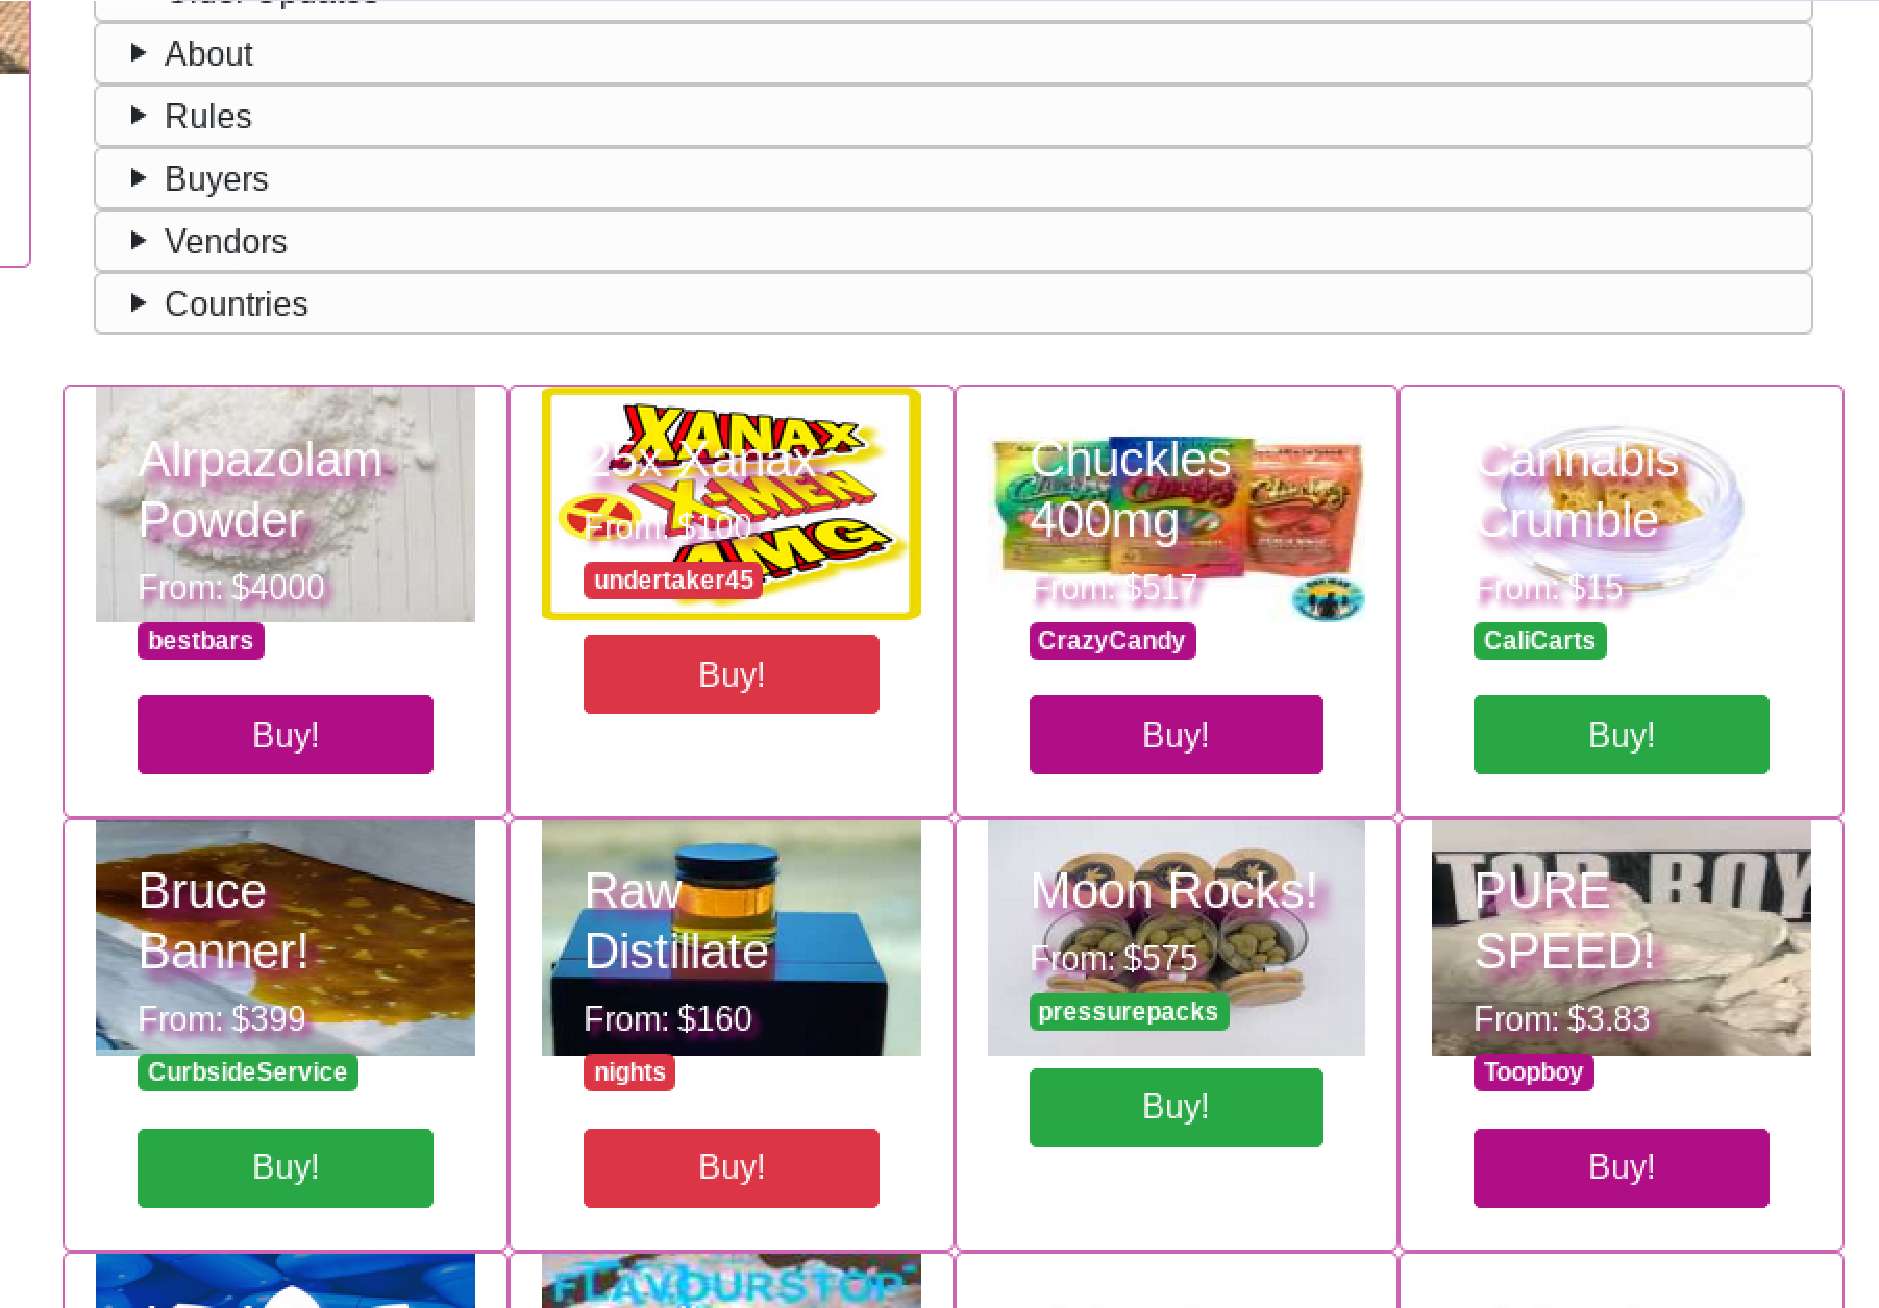
\includegraphics[width=0.8\columnwidth]{dkwb.pdf}}
\caption{Dark Market}\label{fig:dkwb}
\end{figure}


\textbf{Caution:} While browsing the dark webs, you must:   
\begin{itemize}
\item Some dark webs may require registration before accessing their contents. Please do not provide any personal information. 
\item Always use your alias to communicate with other people in dark webs. 
\item Please do not buy anything from dark webs.
\item Please do not visit illegal content (e.g., child porn) on the dark webs.
\end{itemize}

\textbf{Question 1.} Put a screenshot into your report to show you have launched one of the dark webs successfully (10 points). 

\textbf{Question 2.} Copy one of the dark web addresses to your the address bar of  \textsf{Firefox} and check if you can visit the address. If not, explain why. If yes, put a screenshot into your report (10 points). 

\item Open your \textsf{Firefox} and visit \url{https://whatismyipaddress.com/} to check your IP address. Please remember this IP address, and we will use it later.   

 
\item Open your \torbw and visit \url{https://whatismyipaddress.com/} to check your IP address again.  

\textbf{Question 3.} Are the IP addresses displayed in the step 4 and step 5 the same? If not, explain why (10 points). 

\item  Close your \textsf{Firefox}  and relaunch it again. Go to \url{https://whatismyipaddress.com/} to check your IP address.  

\item Close your \torbw and relaunch it again. Go to \url{https://whatismyipaddress.com/} to check your IP address again. 

\textbf{Question 4.} Are the IP addresses displayed in the step 4 and step 6 the same? If not, explain why (10 points).  

\textbf{Question 5.} Are the IP addresses displayed in the step 5 and step 7 the same? If not, explain why (10 points). 

 
\end{enumerate}

\section{Task~3: Understanding \tor via ``whois'' command (20 points)} 
\begin{enumerate}
\item Install \textsf{whois}. Whois is a tool for searching the specific information (e.g., current registrar, registrant information) of a specific domain, 
 \begin{lstlisting}
$ apt install whois
\end{lstlisting}\vspace{-6mm}
\item Check the information about \texttt{osu.edu}
 \begin{lstlisting}
$ whois osu.edu
\end{lstlisting}\vspace{-6mm}

\textbf{Question 1.} Put a screenshot into your report to show you have checked the information about \texttt{osu.edu} (10 points). 

\item Check the IP address of yourself (the IP address obtained in Task.2, step 4) using \textsf{whois}.

\item Check the IP address of IP addresses displayed in \torbw (i.e., the IP addresses displayed in Task2, Step 5 and Task 2, Step 7) using \textsf{whois}.

\textbf{Question 2.} Put a screenshot into your report to show you have checked the IP addresses displayed in \torbw. Explain what you observed (10 points). 

Please note that the IP addresses displayed can be either an IPV4 address or an IPV6 address, and \textsf{whois} can handle both.  

\end{enumerate}

\section{Task~4: Understanding \tor via \tor services (30 points)} 
\begin{enumerate}
\item Install \tor services, which can anonymize all the traffic from your machine.
 \begin{lstlisting}
$ sudo apt install tor
\end{lstlisting}\vspace{-6mm}
\item You can start \tor services using the following commands: 
 \begin{lstlisting}
$ sudo service tor start
\end{lstlisting}\vspace{-6mm}




\item Check the status of your \tor services:
 \begin{lstlisting}
$ sudo service tor status
\end{lstlisting}\vspace{-6mm}

\textbf{Question 1.} Put a screenshot into your report to show \tor services have launched successfully (10 points). 


\item You can also check the running status of \tor services by visiting the following URL in a \textsf{Firefox}: http://127.0.0.1:9050 .

\begin{figure}[h]
\centering
\frame{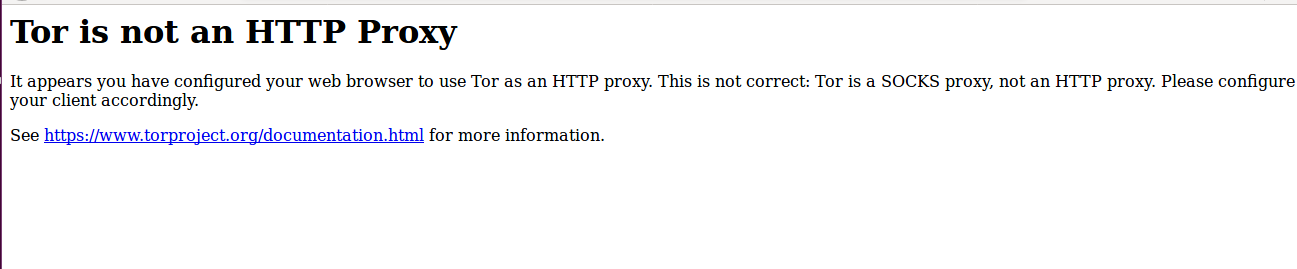
\includegraphics[width=0.8\columnwidth]{proxy.png}}
\caption{Check running status of the tor by using {\sf Firefox}}\label{fig:proxy}
\end{figure}

\item Configure your \textsf{Firefox} as follows. By doing that, we will use \tor services to tunnel the traffic (See \autoref{fig:proxyenable}). 

\begin{figure}[h]
\centering
\frame{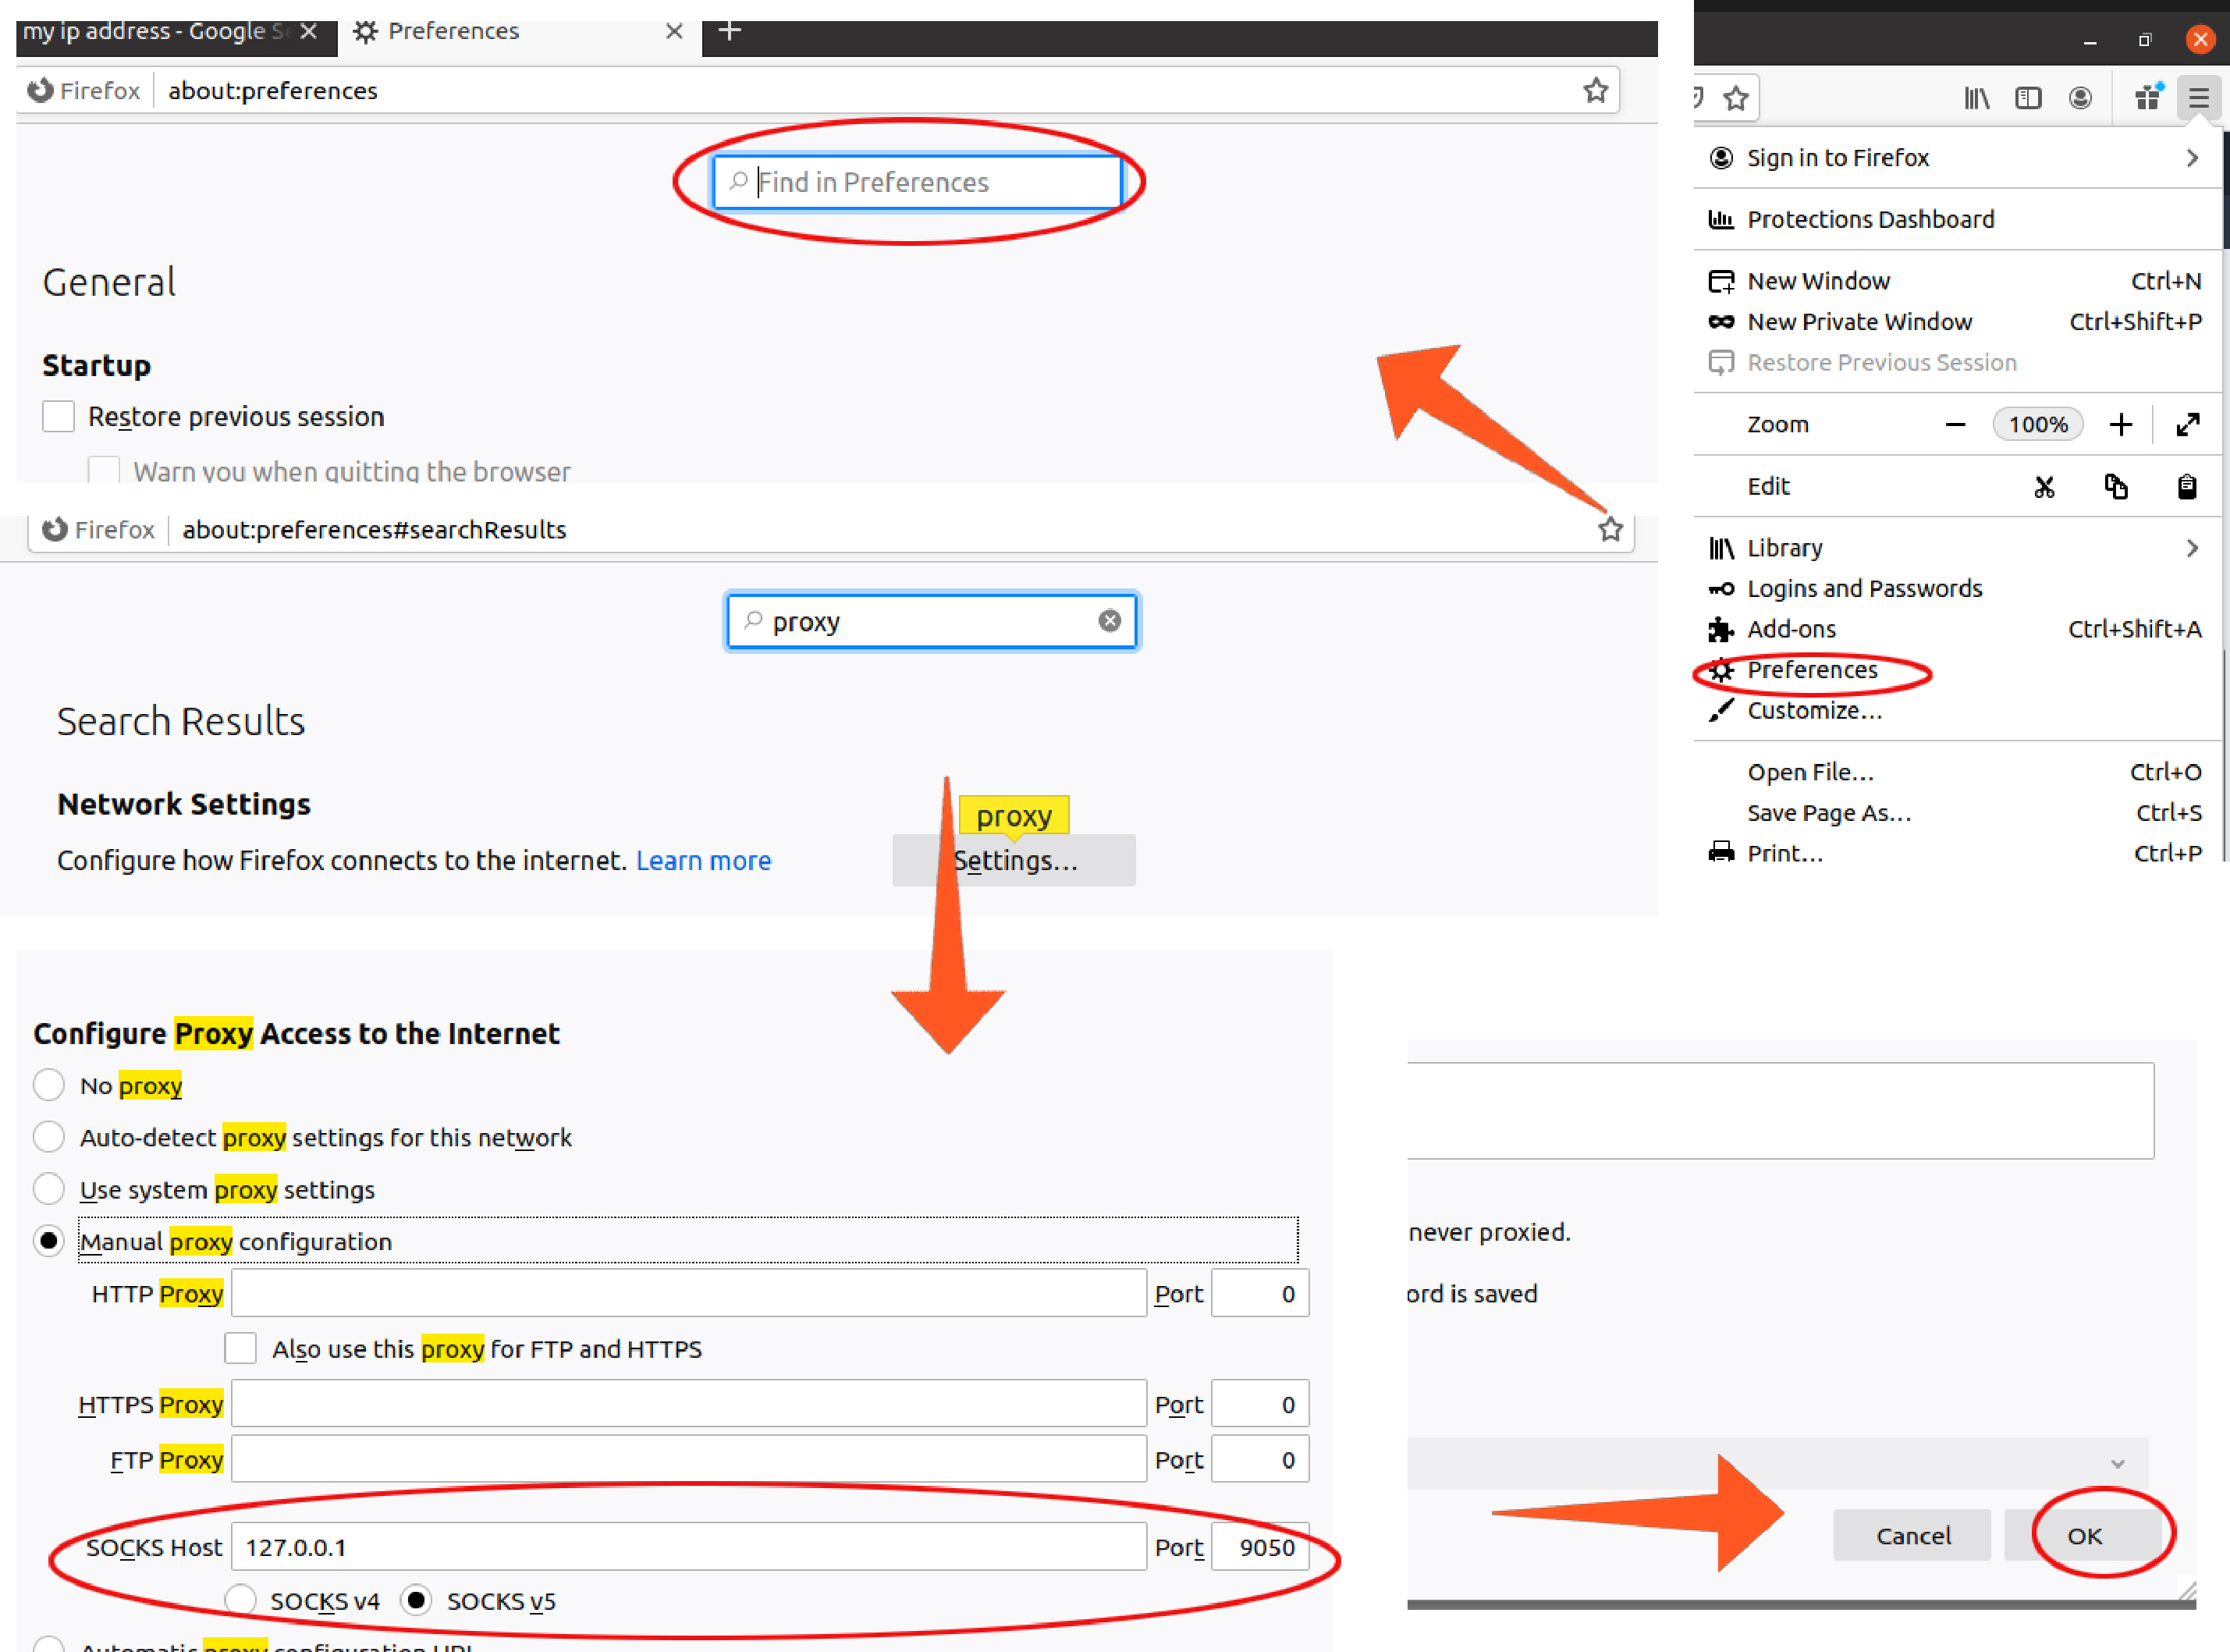
\includegraphics[width=0.8\columnwidth]{proxyenable.pdf}}
\caption{Enabling Proxy}\label{fig:proxyenable}
\end{figure}

\item Use your \textsf{Firefox} to visit \url{https://whatismyipaddress.com/} to check your IP address.  

\textbf{Question 2.} Put a screenshot into your report to show the IP address displayed in your \textsf{Firefox} and explain why (10 points).

\item Stop the \tor services using following command and disable Poxy (See \autoref{fig:proxydisable})
 \begin{lstlisting}
$ sudo service tor stop
\end{lstlisting}\vspace{-6mm}

\begin{figure}[h]
\centering
\frame{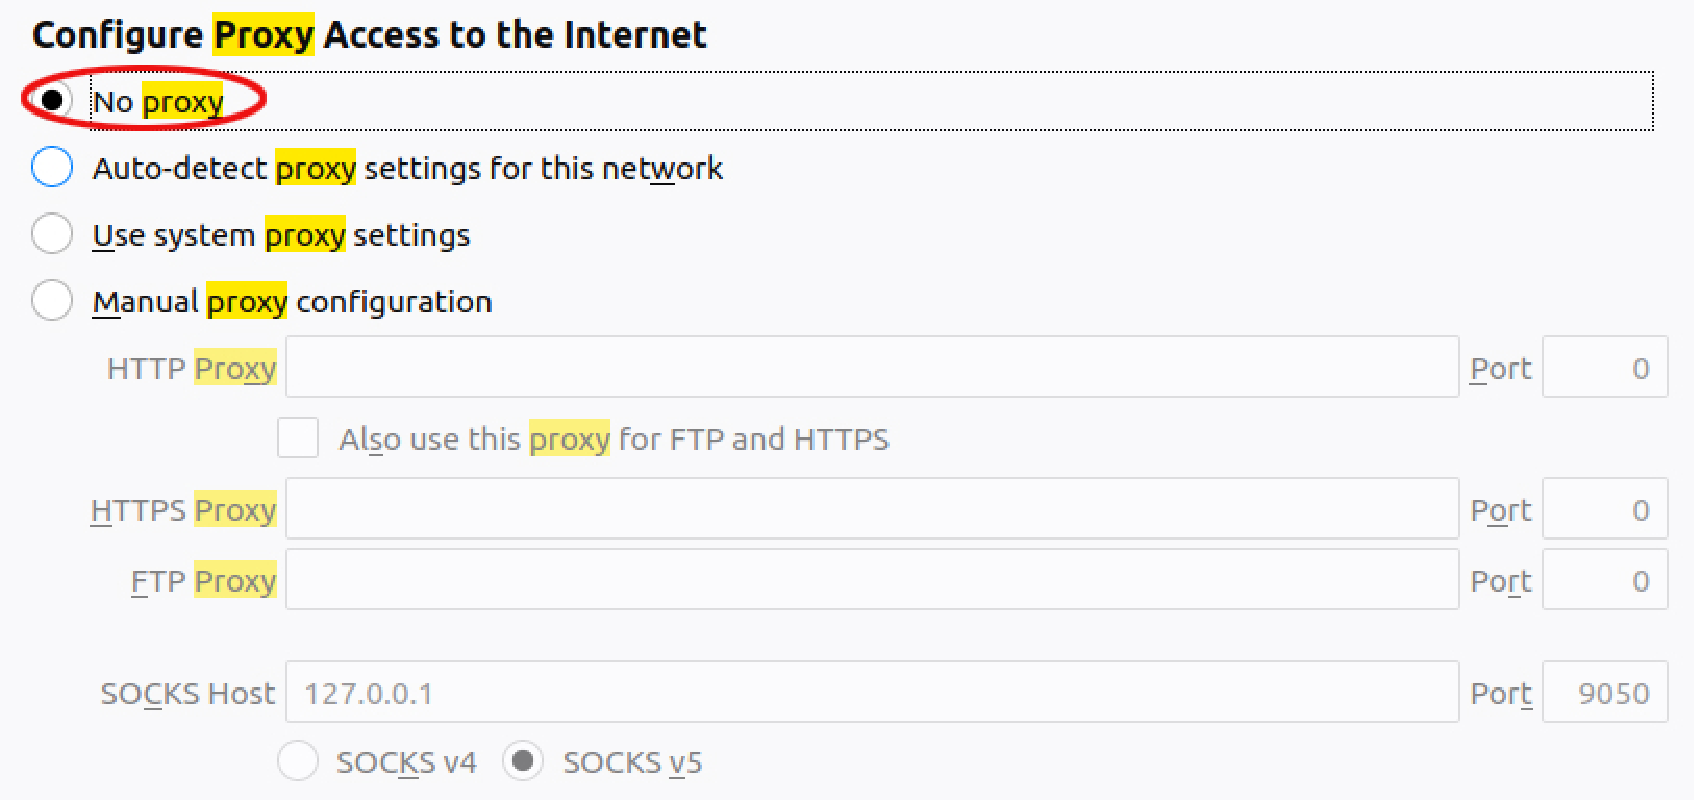
\includegraphics[width=0.8\columnwidth]{proxydisable.pdf}}
\caption{Disabling Proxy}\label{fig:proxydisable}
\end{figure}

\item Use your \textsf{Firefox} to visit \url{https://whatismyipaddress.com/} to check your IP address.

\textbf{Question 3.}  Are the IP addresses displayed in the step 6 and step 8 the same? If not, explain why (10 points). 

\end{enumerate}




%\section{Description}
%\begin{enumerate}
%\item \textbf{SQL injection} vulnerabilities are very serious flaws which open applications up to a whole host of database attacks. These vulnerabilities affect more than just web based applications and often allow the circumvention of authentication/access controls for information stored in a database. Also, SQL injection flaws can sometimes be a stepping stone used by attackers to fully compromise a database server. You could find more information about SQL injection in Section~\ref{reference}.

%\item \textbf{Cross-site scripting} vulnerabilities are also quite common in web applications. These flaws allow you to expose the interaction between users and a website. Read more about the different forms of XSS and how they are typically exploited through the provided references in Section~\ref{reference}.

%\item \textbf{Shell command injection}: while somewhat rare, can be devastating to an application's security because these kinds of flaws generally allow remote execution of code and are usually easy to exploit.The problem usually lies in an application's use of external commands to accomplish certain tasks. Often, for the convenience of it, programmers will run external commands via the system shell or some equivalent interface. However, if a user input is included in such commands (for instance, as command line parameters), then it is very difficult to prevent shell meta-character injection. Read more about these attacks and how they can be prevented in Section~\ref{reference}.\end{enumerate} \section{Set up the environmen
 

  


\section{Submit Your Lab Report}
\label{deliver}
Please write a report describing how you solve each of the problem above, and submit at CARMEN.

\section{Code of Conduct}

These labs are intended for educational purposes only, to provide a safe and legal means to gain an understanding of security by understanding threats and vulnerabilities. They are not intended for (and are not to be used for) any purposes other than for education. 

Some of these labs are based on existing exploits, and students are to exploit their own virtual machines ONLY. Do not try them outside your personal devices. Use of anything learned in, during, or resulting from this class that is in any manner illegal, unauthorized, or unethical is forbidden. There are serious consequences for illegal computer hacking. Any student who violates the rules is subject to legal action, will take sole responsibility of his/her actions, and cannot hold any claim on the responsibility of the faculty, staff, or the university. Students who violate these conditions of the labs will get a failing grade in the class and may be subject to legal action. 
Do not incorporate or implement viruses, worms, spyware and/or Trojan horses in ANY of these labs. Only the tools and resources specified in the given lab may be used. Any student who exploits fellow student's accounts or gains the solutions to the labs by means other than specified is engaging in academic misconduct. Academic misconduct will be treated seriously. 



\end{document}

